\label{sec:ed}
The TU/e \acrfull{ed} is a \acrfull{ros} based 3D geometric, object-based world representation system for robots. ED is a database system that structures multi-modal sensor information and represents this such that it can be utilized for robot localisation, navigation, manipulation and interaction. Figure \ref{fig:ed} shows a schematic overview of ED.

ED has been used on our robots in the OPL since 2012 and was also used this year in the DSPL. Previous developments have focused on making ED platform independent, as a result ED has been used on the PR2, Turtlebot, Dr. Robot systems (X80), as well as on multiple other @Home robots.
\begin{figure}[h]
    %\vspace{-0.3cm}
	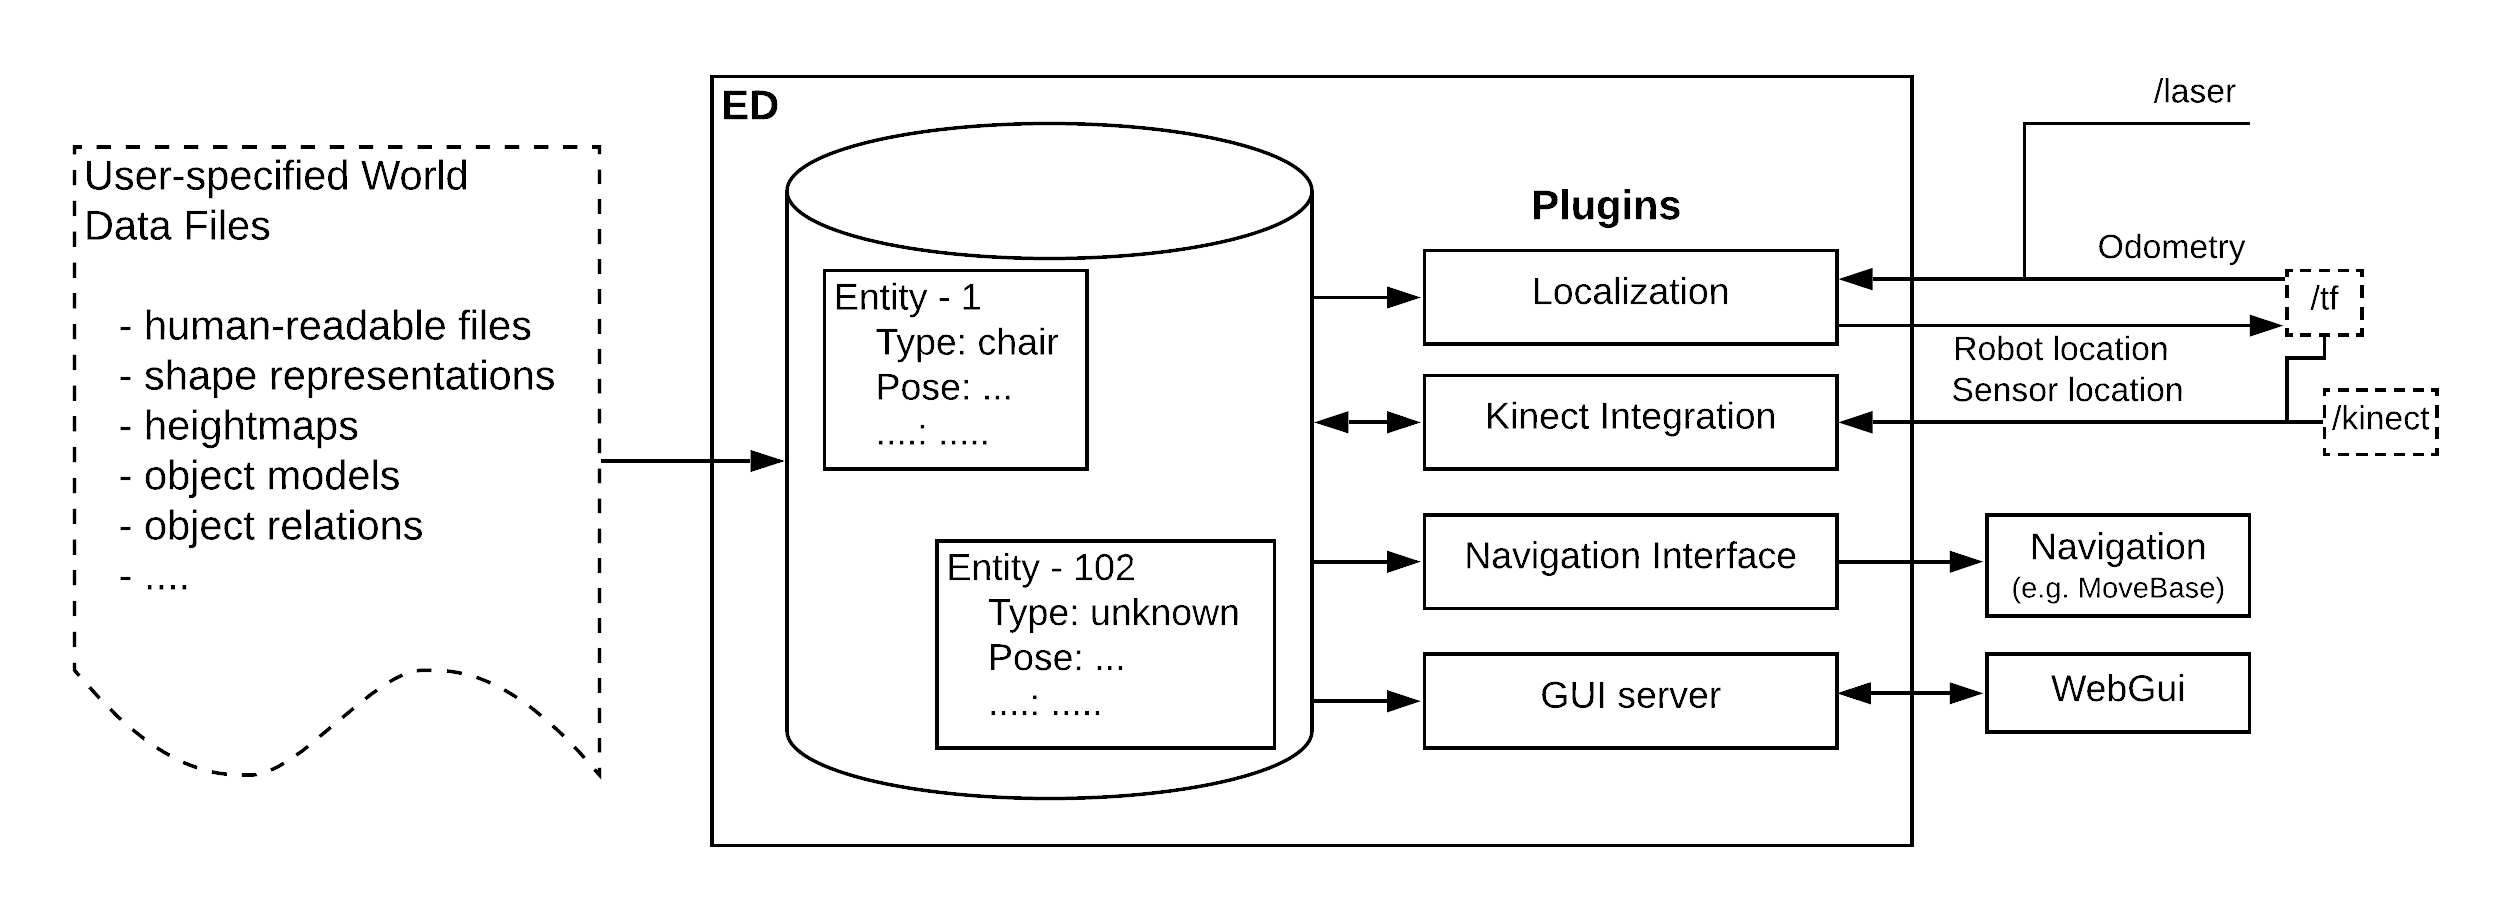
\includegraphics[width = 0.9\linewidth]{Figures/ed_overview}
    %\vspace{-1em}
	\caption{Schematic overview of TU/e Environment Descriptor. Double sided arrows indicate that the information is shared both ways, one sided arrows indicate that the information is only shared in one direction.}
	\label{fig:ed}
    %\vspace{-0.5cm}
\end{figure}
ED is a single re-usable environment description that can be used for a multitude of desired functionalities such as object detection, navigation and human machine interaction. Improvements in ED reflect in the performances of the separate robot skills, as these skills are closely integrated in ED. It omits updating and synchronization of multiple world models. Currently, different \acrshort{ed} plug-ins exist that enable robots to localize themselves, update positions of known objects based on recent sensor data, segment and store newly encountered objects and visualize all this in RViz and through a web-based \acrshort{gui}, as illustrated in Figure \ref{fig:gui_actions}.
\begin{figure}[h]
\centering
    %\vspace{-0.3cm}
	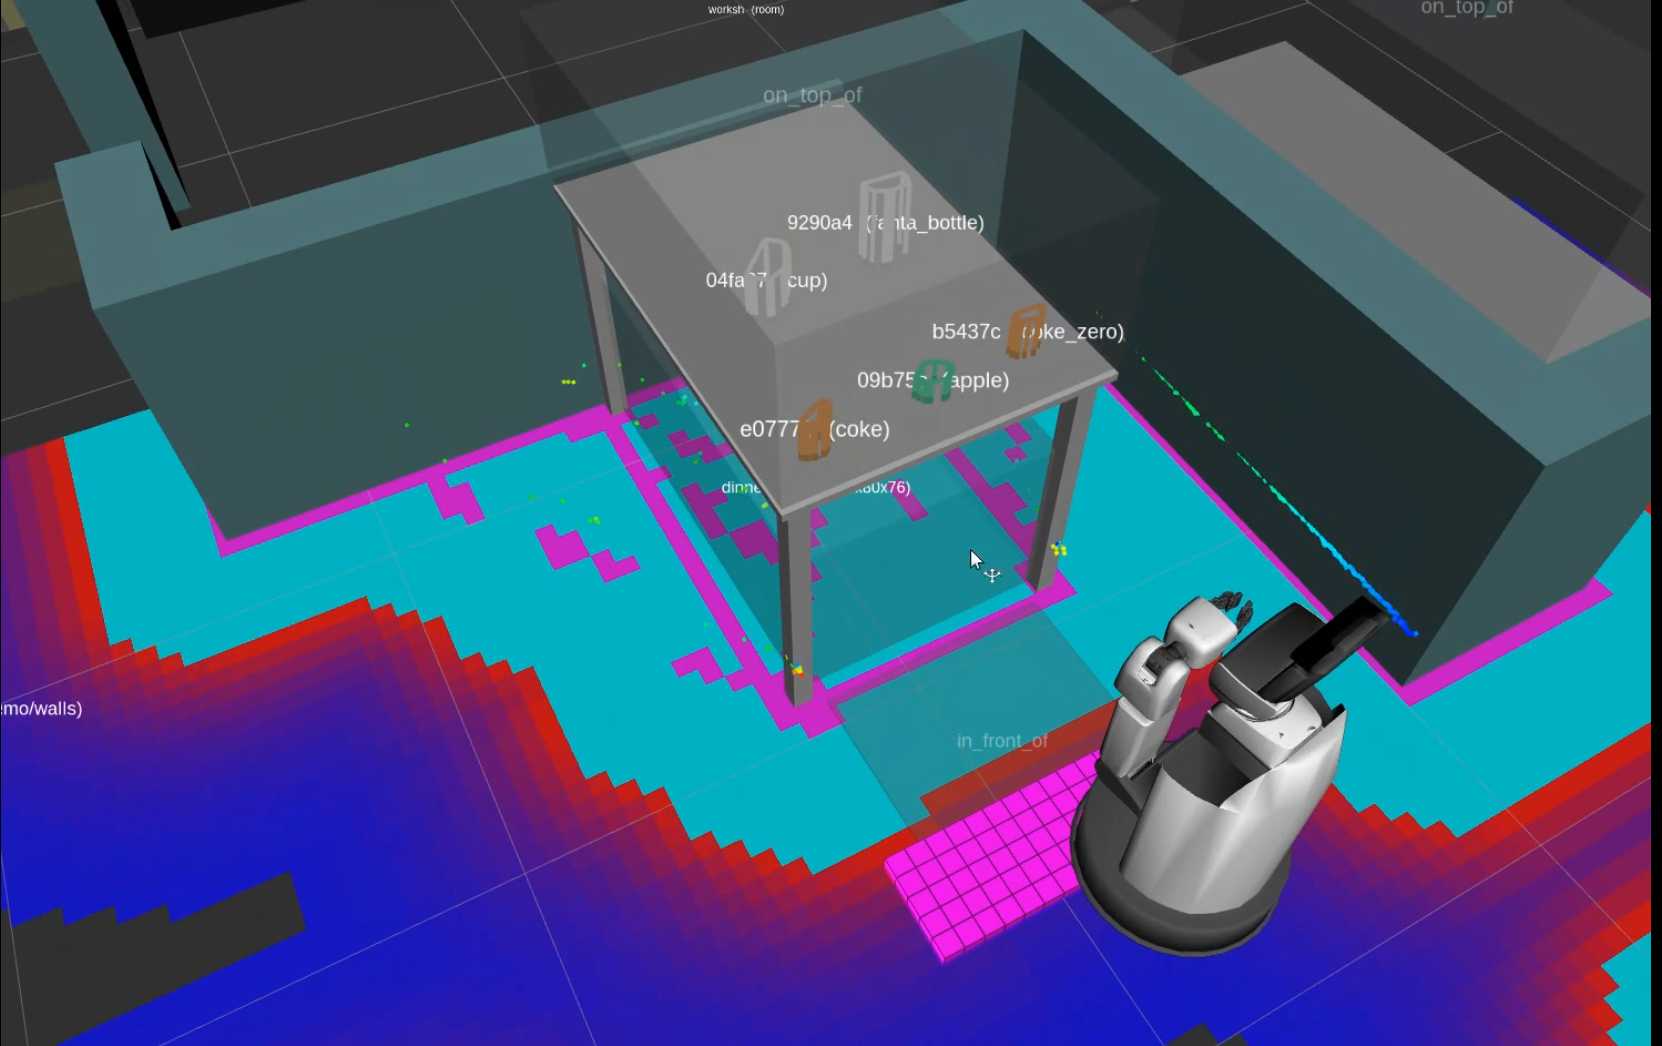
\includegraphics[width = 0.8\linewidth]{Figures/ed_segmentation_hsr}
    %\vspace{-0.5em}
	\caption{A view of the world model created with \acrshort{ed}. The figure shows the occupancy grid as well as classified objects recognized on top of the cabinet.}
	\label{fig:ed_segmentation}
    %\vspace{-0.5cm}
\end{figure}
